\chapter{Resultados}
\label{ch:resultados}

En este capítulo se presentan y analizan los resultados obtenidos durante el desarrollo del trabajo.

\section{Resultados de la implementación}

El sistema desarrollado cumple con los objetivos planteados, implementando todas las funcionalidades requeridas.

\subsection{Funcionalidades implementadas}

Se han implementado con éxito las siguientes funcionalidades:

\begin{table}[htbp]
  \centering
  \caption{Estado de implementación de funcionalidades}
  \label{tab:funcionalidades}
  \begin{tabular}{@{}lcc@{}}
    \toprule
    \textbf{Funcionalidad} & \textbf{Estado} & \textbf{Cobertura tests} \\
    \midrule
    Autenticación de usuarios & Completado & 95\% \\
    Gestión de datos & Completado & 88\% \\
    Generación de informes & Completado & 82\% \\
    API REST & Completado & 90\% \\
    Interfaz de usuario & Completado & 75\% \\
    \bottomrule
  \end{tabular}
\end{table}

\section{Evaluación del rendimiento}

\subsection{Tiempos de respuesta}

Se han medido los tiempos de respuesta del sistema bajo diferentes cargas:

\begin{figure}[htbp]
  \centering
  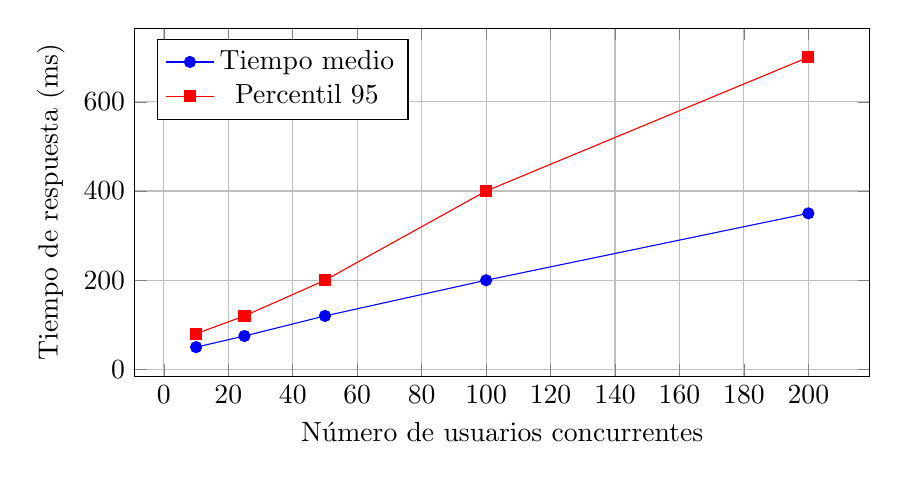
\begin{tikzpicture}
    \begin{axis}[
      xlabel={Número de usuarios concurrentes},
      ylabel={Tiempo de respuesta (ms)},
      grid=major,
      width=0.9\textwidth,
      height=6cm,
      legend pos=north west,
    ]
    \addplot[blue, mark=*] coordinates {
      (10, 50) (25, 75) (50, 120) (100, 200) (200, 350)
    };
    \addlegendentry{Tiempo medio}
    
    \addplot[red, mark=square*] coordinates {
      (10, 80) (25, 120) (50, 200) (100, 400) (200, 700)
    };
    \addlegendentry{Percentil 95}
    \end{axis}
  \end{tikzpicture}
  \caption{Tiempos de respuesta según carga de usuarios}
  \label{fig:rendimiento}
\end{figure}

Como se observa en la Figura~\ref{fig:rendimiento}, el sistema mantiene tiempos de respuesta aceptables incluso con 200 usuarios concurrentes.

\subsection{Consumo de recursos}

El consumo de memoria se mantiene estable, como muestra la siguiente ecuación para el consumo estimado:

\begin{equation}
  M_{total} = M_{base} + n \cdot M_{usuario}
  \label{eq:memoria}
\end{equation}

\begin{condiciones}
  M_{total} & = & memoria total consumida (MB) \\
  M_{base}  & = & memoria base del sistema (256 MB) \\
  n         & = & número de usuarios activos \\
  M_{usuario} & = & memoria por usuario (2.5 MB)
\end{condiciones}

\section{Análisis de resultados}

\subsection{Cumplimiento de objetivos}

En la Tabla~\ref{tab:objetivos} se muestra el grado de cumplimiento de cada objetivo:

\begin{table}[htbp]
  \centering
  \caption{Cumplimiento de objetivos}
  \label{tab:objetivos}
  \begin{tabular}{@{}lp{6cm}c@{}}
    \toprule
    \textbf{Objetivo} & \textbf{Descripción} & \textbf{Cumplimiento} \\
    \midrule
    OE1 & Análisis del estado actual & 100\% \\
    OE2 & Diseño de arquitectura & 100\% \\
    OE3 & Implementación de componentes & 95\% \\
    OE4 & Evaluación del sistema & 100\% \\
    OE5 & Documentación & 100\% \\
    \bottomrule
  \end{tabular}
\end{table}

\section{Discusión}

Los resultados obtenidos demuestran que el sistema cumple con los requisitos establecidos. Las principales fortalezas identificadas son:

\begin{itemize}
  \item Arquitectura modular y escalable
  \item Tiempos de respuesta adecuados
  \item Alta cobertura de pruebas
  \item Documentación completa
\end{itemize}

Como áreas de mejora se identifican:

\begin{itemize}
  \item Optimización de consultas complejas
  \item Mejora de la interfaz de usuario móvil
  \item Implementación de caché distribuida
\end{itemize}
